
\subsection{Vlastní čísla grafu}

\df Vlastní čísla grafu jsou vlastní čísla matice sousednosti grafu. Množina 
vlastních čísel je {\it spektrum}, $\Sp = \{\lambda_1, \lambda_2, \dots\}$ a 
většinou se udává setříděná podle velikosti (tj. $\lambda_1$ je typicky 
největší vlastní číslo). Pro vlastní čísla platí $Ax = \lambda x$ a lze je 
vypočítat jako $\det(A - \lambda E) = 0$.

\subsection{Expandéry}

\vt (O vlastních číslech bipartitního grafu) Graf $G$ je bipartitní právě 
tehdy, když je jeho spektrum symetrické (vzhledem k nule). Pokud je navíc $G$ 
souvislý, stačí pouze $\lambda_{min} = -\lambda_{max}$.

\df Rodina expandérů $G_i$ je třída d-regulárních grafů rostoucích velikostí, 
kde každý graf má \uv{dobrou expanzí} (podle nějakého parametru).

\df (Expanze) \begin{itemize}
	\item Vrcholová expanze: $h_v(G) = \min_{S\subseteq V, |S|\leq n/2} 
	{|N(S)\setminus S| \over |S|}$.
	\item Hranová expanze: $h(G) = \min_{S\subseteq V, |S|\leq n/2} {|\delta S| 
	\over |S|}$, kde $\delta S$ značí hrany, které mají právě jeden vrchol v 
	$S$.
\end{itemize}

\poz (O hranové a vrcholové expanzi) $h_v(G) \leq h(G) \leq d \cdot h_v(G)$.

\vt (O vlastních číslech a expanzi) Pro $G$ $d$-regulární graf platí: $1/2(d - 
\lambda_2) \leq h(G) \leq \sqrt{d \cdot (d - \lambda_2)}$

\subsection{Konstrukce expandérů}

Ačkoliv například úplný graf je dobrý expandér ve smyslu, že má vysokou 
expanzi, bohužel s expanzí a velikostí roste neúnosně stupeň. Následující 
konstrukce vytváří grafy, které mají vyokou expanzi, ale konstantně malý 
stupeň.

\vt (Randomizovaná) Mějme $2n$ vrcholů. Pro $d$-regulární expandér zvolíme $d$ 
uniformě náhodných prefektních párování nad těmito vrcholy. Sjednocení těchto 
párování dává $d$-regulární graf, který je navíc dobrý expandér.

\vt (Prvočíselná) Nechť $p$ je prvočíslo a $V:=Z_p$. Definujeme $G_p=(V,E)$ s 
hranami $(x, x+1)$ a $(x,x^{-1})$ ($0^{-1}$). Pak $G_p$ je rodina dobrých 
expandérů.

\vt (Margulis) Nechť $G_m=(V,E)$ a $V=\Z_m \times \Z_M$. Definujeme hrany pro 
$4$-regulární graf jako: $(x\pm y, y)$ a $(x,y\pm x)$. Pak $G_m$ je rodina 
dobrých expandérů.

\df (Zig-Zag) Nechť $G$ je $g$-regulární graf a $H$ je $h$-regulární graf na $d$ 
vrcholech. Definujeme $G \zz H$ následujícím způsobem:
\begin{enumerate}
	\item Říkejme, že hrany z $G$ jsou {\bf\color{red}červené} a hrany z $H$ 
		jsou {\bf\color{blue}modré}.
	\item Vrcholy $G$ nahradíme grafy $H$ tak, že každému vrcholu $H$ přiřadíme 
	jednu hranu $G$. Protože $G$ je $g$-regulární a $H$ má právě $g$ vrcholů, 
	nyní každý vrchol má právě jednu hranu z $G$.
	\item Pro každou cestu tvaru 
		{\bf\color{blue}modrá}-{\bf\color{red}červená}-{\bf\color{blue}modrá} 
		vytvoříme {\bf\color{magenta}růžovou} hranu z prvního vrcholu do 
		posledního vrcholu.
	\item Odstraníme z grafu {\bf\color{blue}modré}-{\bf\color{red}červené} 
		hrany.
\end{enumerate}
Ukázka konstrukce je na obrázku \ref{zigzag-konstrukce}. Pro názornost není graf
$H$ regulární (nepodařilo se mi najít lepší příklad). Příklad je převzat z webu
\footnote{
\url{http://math.stackexchange.com/questions/454162/clearing-doubt-over-a-definition}}.

\begin{figure}
\centering
\begin{subfigure}{7.5cm}{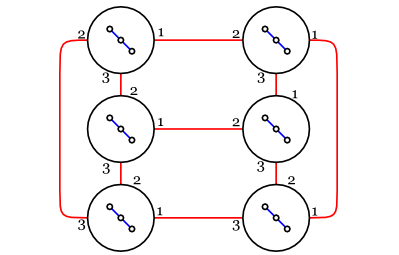
\includegraphics[width=\textwidth]{img/zigzag1.png}}\caption{Vložení 
$H$ do $G$}\end{subfigure}
\begin{subfigure}{7.5cm}{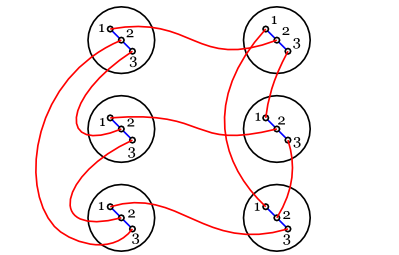
\includegraphics[width=\textwidth]{img/zigzag2.png}}\caption{Napojení 
hran $G$ na vrcholy $H$}\end{subfigure}
\begin{subfigure}{7.5cm}{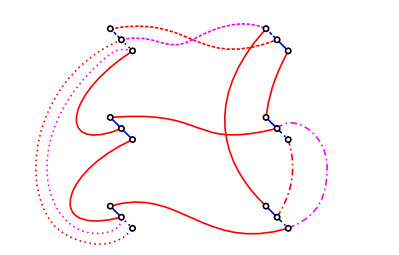
\includegraphics[width=\textwidth]{img/zigzag3.png}}\caption{Tvorba 
růžových hran}\end{subfigure}
\begin{subfigure}{7.5cm}{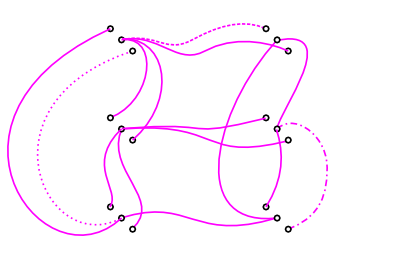
\includegraphics[width=\textwidth]{img/zigzag4.png}}\caption{Výsledek}\end{subfigure}
\caption{Příklad Zig-Zag součinu. Pro jednoduchost není $H$ regulární, na funkci
to ale nic nemění.}
\label{zigzag-konstrukce}
\end{figure}

\poz Díky této konstrukci máme graf, který zachovává velikost $G$ (dokonce ji 
zvětšuje), ale dědí stupeň po grafu $H$ (pokud stupeň byl $h$, nyní bude $h^2$ 
-- to sice není úplně dobré, ale mohlo by to být horší).

\vt (Zig-Zag) Nechť $H$ je dobrý $d$-regulární expandér, $G_1 := H^2$. Potom 
rodina grafů $G_{i+1} := G_i\zz H$ je dobrý expandér.
